\documentclass[tikz,border=5pt]{standalone}
\usepackage{fontspec}
\setmainfont{Times New Roman}
\usepackage{unicode-math}
\setmathfont{Cambria Math}
\usetikzlibrary{shapes.geometric,positioning,fit,backgrounds,arrows.meta,calc}

\begin{document}
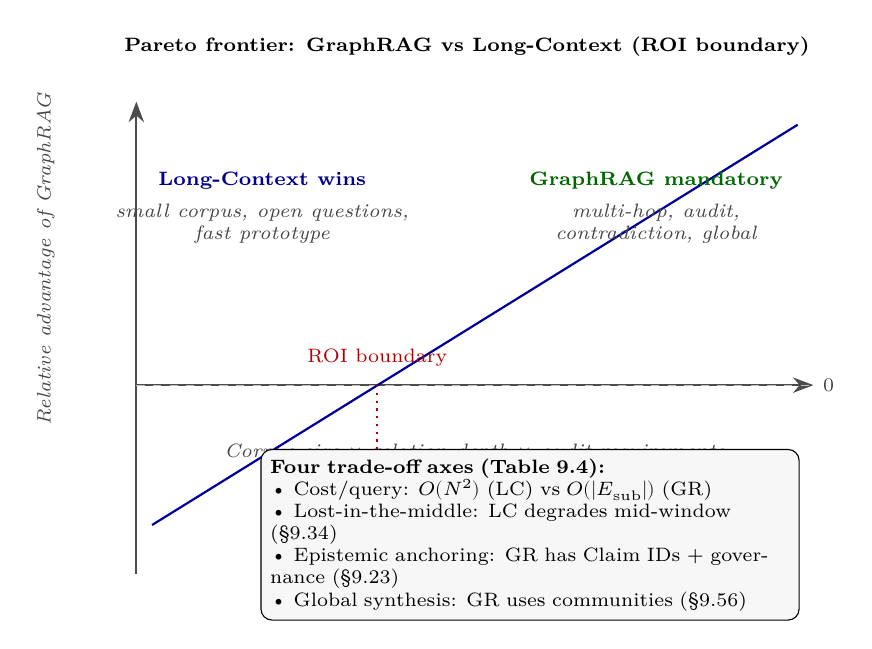
\begin{tikzpicture}[
  axis/.style={-{Stealth[length=2.6mm]}, thick, gray!60!black},
  curve/.style={thick, blue!60!black},
  label/.style={font=\scriptsize\itshape, text=gray!55!black},
  reg/.style={font=\scriptsize\bfseries},
]

% === Title ===
\node[font=\scriptsize\bfseries] at (4.2, 4.3) {Pareto frontier: GraphRAG vs Long-Context (ROI boundary)};

% === Axes ===
\draw[axis] (0,0) -- (8.6,0) node[right, font=\scriptsize, text=gray!60!black] {};
\draw[axis] (0,-2.4) -- (0,3.6);

% X label
\node[label, align=center] at (4.3, -1.0) {Corpus size $\times$ relation depth $\times$ audit requirements\\
 (problem difficulty)};
% Y label
\node[label, rotate=90, align=center] at (-1.15, 1.6) {Relative advantage of GraphRAG};

% zero line
\draw[dashed, gray!50] (0,0) -- (8.6,0);
\node[label, right] at (8.6, 0) {$0$};

% === Rising curve crossing zero at ROI boundary ===
\draw[curve] plot[smooth, domain=0.2:8.4, samples=60]
  (\x, {-1.9 + 0.62*\x});

% ROI boundary marker
\draw[dotted, thick, red!70!black] (3.06,0) -- (3.06,-2.4);
\node[font=\scriptsize, text=red!70!black] at (3.06, 0.35) {ROI boundary};

% === Region labels ===
\node[reg, text=blue!55!black] at (1.6, 2.6) {Long-Context wins};
\node[label, align=center] at (1.6, 2.05) {small corpus, open questions,\\fast prototype};

\node[reg, text=green!40!black] at (6.6, 2.6) {GraphRAG mandatory};
\node[label, align=center] at (6.6, 2.05) {multi-hop, audit,\\contradiction, global};

% === Four Pareto axes legend (bottom-right box) ===
\node[draw, rounded corners, fill=gray!6, align=left, font=\scriptsize, text width=6.6cm] (leg) at (5.0, -1.9)
  {\textbf{Four trade-off axes (Table 9.4):}\\
   \textbullet\ Cost/query: $O(N^2)$ (LC) vs $O(\lvert E_{\text{sub}}\rvert)$ (GR)\\
   \textbullet\ Lost-in-the-middle: LC degrades mid-window (§9.34)\\
   \textbullet\ Epistemic anchoring: GR has Claim IDs + governance (§9.23)\\
   \textbullet\ Global synthesis: GR uses communities (§9.56)};

\end{tikzpicture}
\end{document}